\chapter{Results and Discussion}
\label{sec:results}
This section reports the results of the system proposed in this paper.
The target is considered to be cylindrical in shape considering some of the most statistically-most-concerning (SMC) space debris \cite{mcknight2021identifying} - cylindrical second-stage rocket bodies.
% SL-16s: Zenit second stages that are 4 m in diameter, 12 m in length and 8300 kg in dry mass.
All optimization and optimal control problems are solved using the GEKKO package \cite{beal2018gekko} in Python.
We have used both the Advanced Process OPTimizer (APOPT) \cite{hedengren2014nonlinear} and the Interior Point Optimizer (IPOPT) \cite{wachter2006on} solvers based on the speed and computational resource consumption of each problem.

\section{The Overall Pipeline}
\label{sec:results_pipeline}
We demonstrate in Figure \ref{fig:results_pipeline} the rendezvous and docking of the chaser with the target using ADTMPC.
Here, subfigures \ref{fig:results_x_rnd}, \ref{fig:results_y_rnd}, and \ref{fig:results_z_rnd} demonstrate the positional states of the chaser in the execution of the complete pipeline whereas subfigures \ref{fig:results_x_dock}, \ref{fig:results_y_dock}, and \ref{fig:results_z_dock} focuses on the positional states for the docking operation.
(Note that rendezvous ends and docking begins when the chaser is less than 2.0 units away from the docking position.)
\begin{figure}[H]
  \begin{subfigure}[b]{0.50\textwidth}
    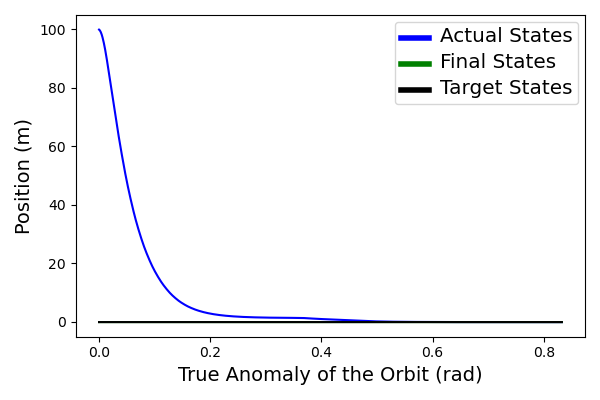
\includegraphics[width=\linewidth]{assets/complete_x_traj.png}
    \caption{Complete Trajectory in the X-axis}
    \label{fig:results_x_rnd}
  \end{subfigure}
  \begin{subfigure}[b]{0.50\textwidth}
    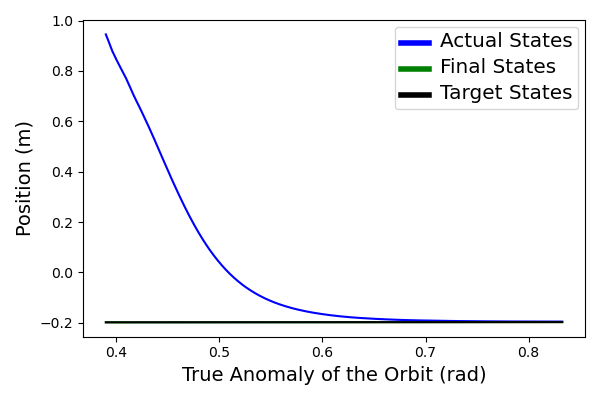
\includegraphics[width=\linewidth]{assets/docking_x_traj.png}
    \caption{Docking Trajectory in the X-axis}
    \label{fig:results_x_dock}
  \end{subfigure}
  \begin{subfigure}[b]{0.50\textwidth}
    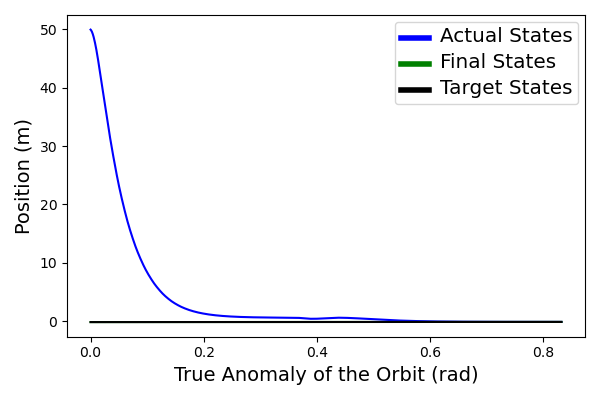
\includegraphics[width=\linewidth]{assets/complete_y_traj.png}
    \caption{Complete Trajectory in the Y-axis}
    \label{fig:results_y_rnd}
  \end{subfigure}
  \begin{subfigure}[b]{0.50\textwidth}
    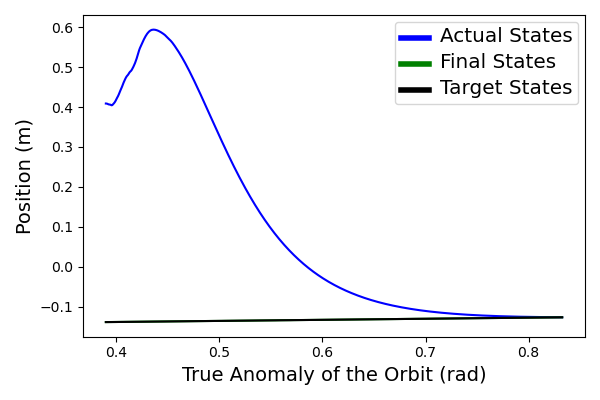
\includegraphics[width=\linewidth]{assets/docking_y_traj.png}
    \caption{Docking Trajectory in the Y-axis}
    \label{fig:results_y_dock}
  \end{subfigure}
  \begin{subfigure}[b]{0.50\textwidth}
    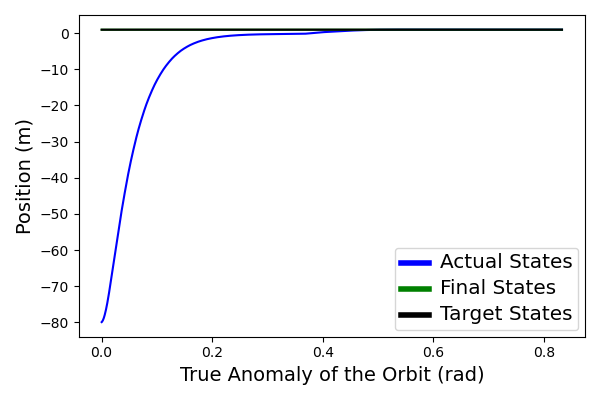
\includegraphics[width=\linewidth]{assets/complete_z_traj.png}
    \caption{Complete Trajectory in the Z-axis}
    \label{fig:results_z_rnd}
  \end{subfigure}
  \begin{subfigure}[b]{0.50\textwidth}
    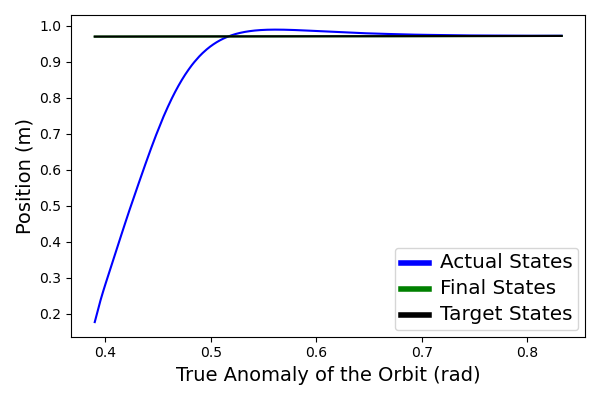
\includegraphics[width=\linewidth]{assets/docking_z_traj.png}
    \caption{Docking Trajectory in the Z-axis}
    \label{fig:results_z_dock}
  \end{subfigure}
  \caption{Simulation of Rendezvous and Docking using ADTMPC}
 \label{fig:results_pipeline}
\end{figure}
The adaptation of the unknown parameters 
- the eccentricity of the orbit and the drag constant of the target - is noted in Table \ref{tab:parameter-estimation} by including the initial and final estimates and ranges of estimation.
We note that it is possible to obtain more precise simulations of the docking operation by adjusting the cost function matrices and other solver parameters; however, we demonstrate the proof-of-concept of the proposed algorithm.
\begin{table}[H]
    \centering
    \resizebox{\textwidth}{!}{\begin{tabular}{|c|c|c|c|c|c|}
    \hline
    Param.                          & Actual Value & Initial Est. & Final Est. & Initial Range & Final Range \\
    \hline
    $\mathsf{e}$         & $\num{1.250e-1}$ & $\num{0.000e-1}$ & $\num{1.2513e-1}$ & $[\num{0.000}, \num{6.000}]\times\num{e-1}$ & $[\num{1.100}, \num{1.373}]\times\num{e-1}$ \\
    $\alpha$ & $\num{1.300e-7}$ & $\num{0.000e-7}$ & $\num{1.2999e-7}$ & $[\num{0.000}, \num{5.000}]\times\num{e-7}$ & $[\num{1.297}, \num{1.326}]\times\num{e-7}$ \\
    \hline
    \end{tabular}}
    \caption{{Estimation of Unknown Parameters via SMID.} This table demonstrates the adaptation of the system to unknown parameters (orbit eccentricity $\mathsf{e}$ and target drag constant $\alpha$) and the shrinking of the estimation ranges.}
    \label{tab:parameter-estimation}
\end{table}
\begin{figure}[H]
  \begin{subfigure}[b]{0.50\textwidth}
    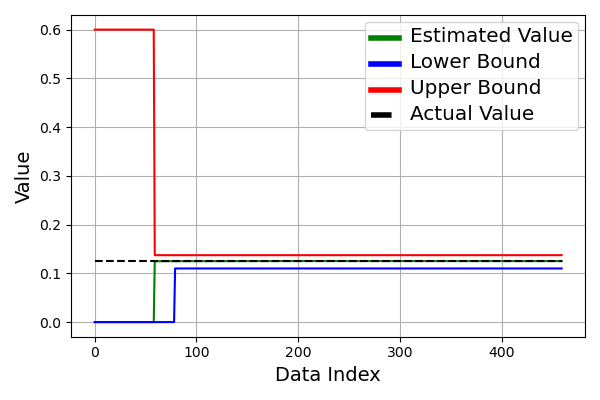
\includegraphics[width=\linewidth]{assets/estim_eccentricity.png}
    \caption{Eccentricity $\mathsf{e}$ of the Orbit}
    \label{fig:results_estim_eccentricity}
  \end{subfigure}
  \hfill
  \begin{subfigure}[b]{0.50\textwidth}
    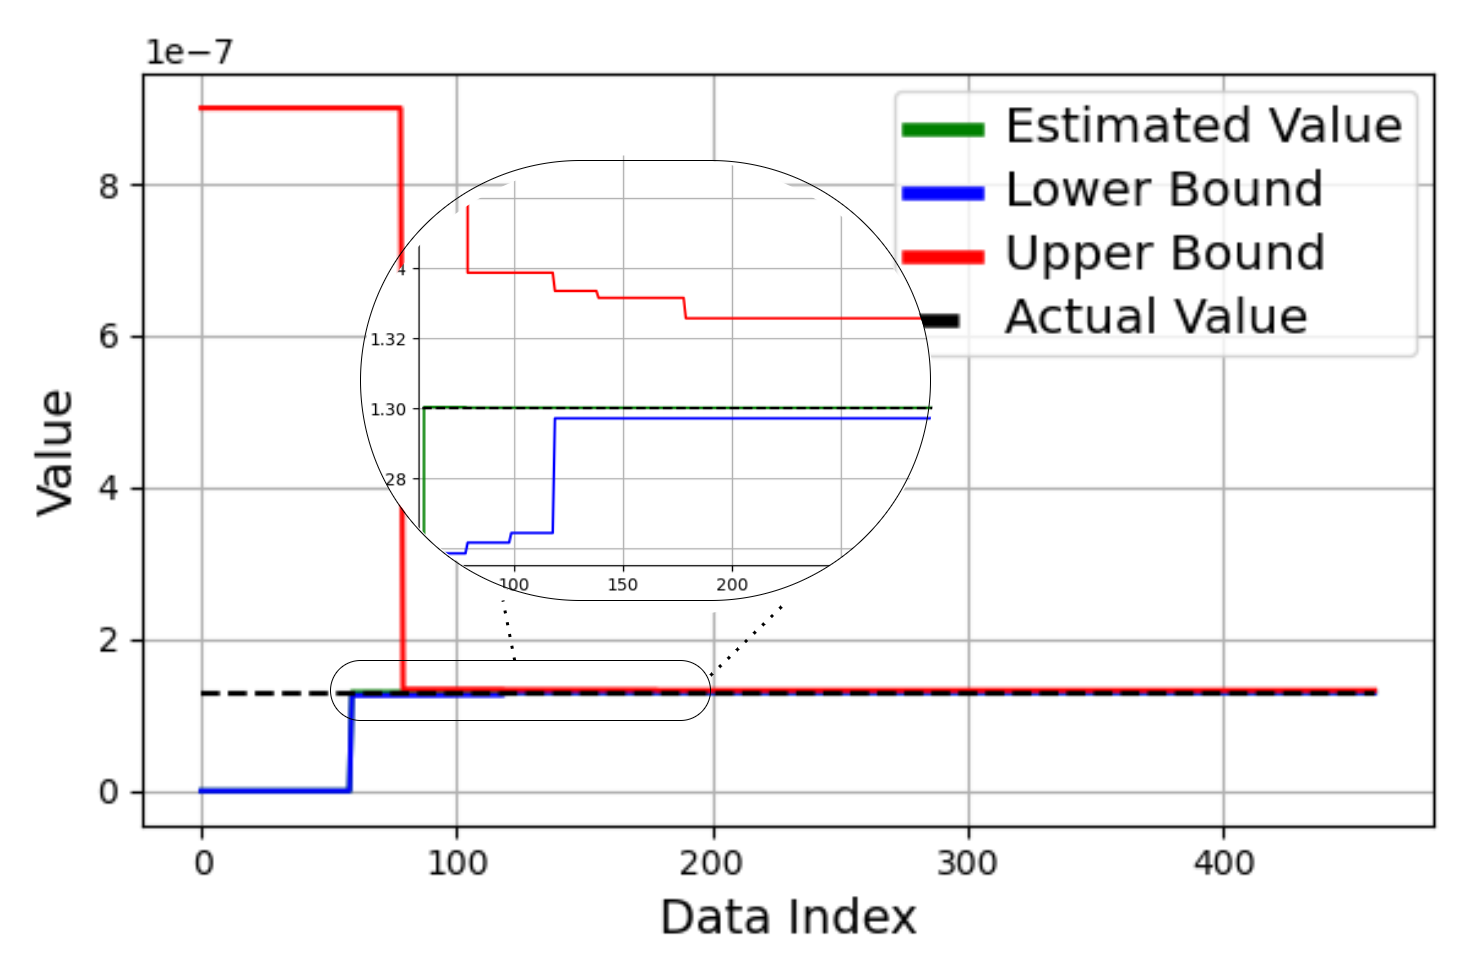
\includegraphics[width=\linewidth]{assets/estim_alpha.png}
    \caption{Drag Constant $\alpha$ of the Target}
    \label{fig:results_estim_alpha}
  \end{subfigure}
  \caption{Estimation of Unknown Parameters via SMID. These figures represent the progress in the estimation of unknown parameters over time using data from the previous MPC iteration.}
  \label{fig:results_estim}
\end{figure}
\subsection{Estimation of Unknown Parameters}
The data in Table \ref{tab:parameter-estimation} and the corresponding plots in Figure \ref{fig:results_estim} demonstrate the estimation of the eccentricity of the orbit and the drag constant of the target from an initial estimate and range to a final estimate that is close to the actual value.
This improves the docking of the chaser due to the corresponding shrinking of the robust tube around the trajectory.
We determine the range and value for eccentricity based on common values of eccentricity for low earth orbits \cite{space2023}.
On the other hand, since this is not easily for target drag constants in orbit, we determine a range and value for this parameter using calculations based on the expression for drag constant and its relation to the standard drag equation \cite{carter2008two,humi2007two}:
\begin{equation}
    F_d=\frac{1}{2}\rho u^2c_dA
\end{equation}
where $F_d$ is the drag force, $\rho$ is the mass density of the fluid, $u$ is the flow velocity relative to the object (in orbit, this can be interpreted as the velocity of the spacecraft), A is the reference area, and $c_d$ is the drag coefficient.

\section{Analysis of ADTMPC and other techniques}
\label{sec:results_analysis}
We perform the following analysis to depict the advantages of using ADTMPC over plain MPC for rendezvous and docking with space debris.
\subsection{Satisfaction of chaser-target collision constraints}
As is visible from Figure \ref{fig:results_tube}, model predictive control without the use of robust tubes leads to the violation of the chaser-target collision constraints in close proximity to the target.
The chaser's trajectory is not able to accurately account for the uncertainties in the target's dynamics and the environment.
In contrast, dynamic tubes help adapt to these uncertainties and maintain a safe distance between the chaser and the target at all times.
\begin{figure}[H]
  \begin{subfigure}[b]{0.49\textwidth}
    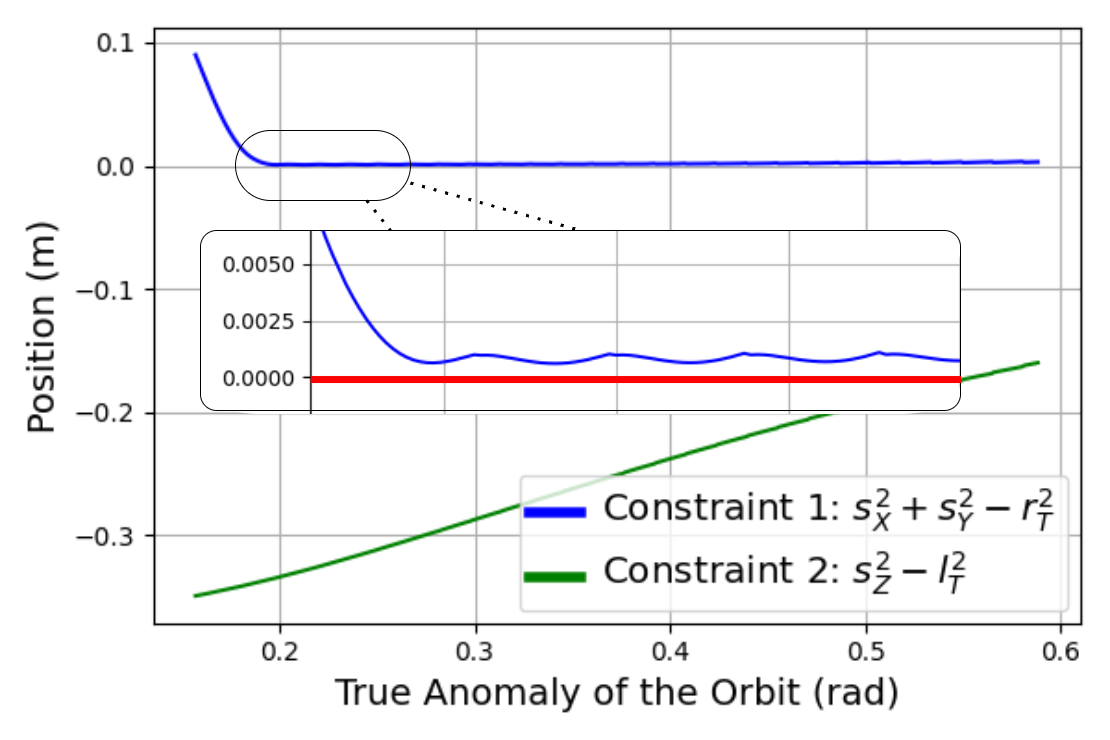
\includegraphics[width=\linewidth]{assets/results_with_tube_dtmpc.png}
    \caption{Dynamic Tube MPC}
    \label{fig:results_with_tube_dtmpc}
  \end{subfigure}
  \hfill
  \begin{subfigure}[b]{0.49\textwidth}
    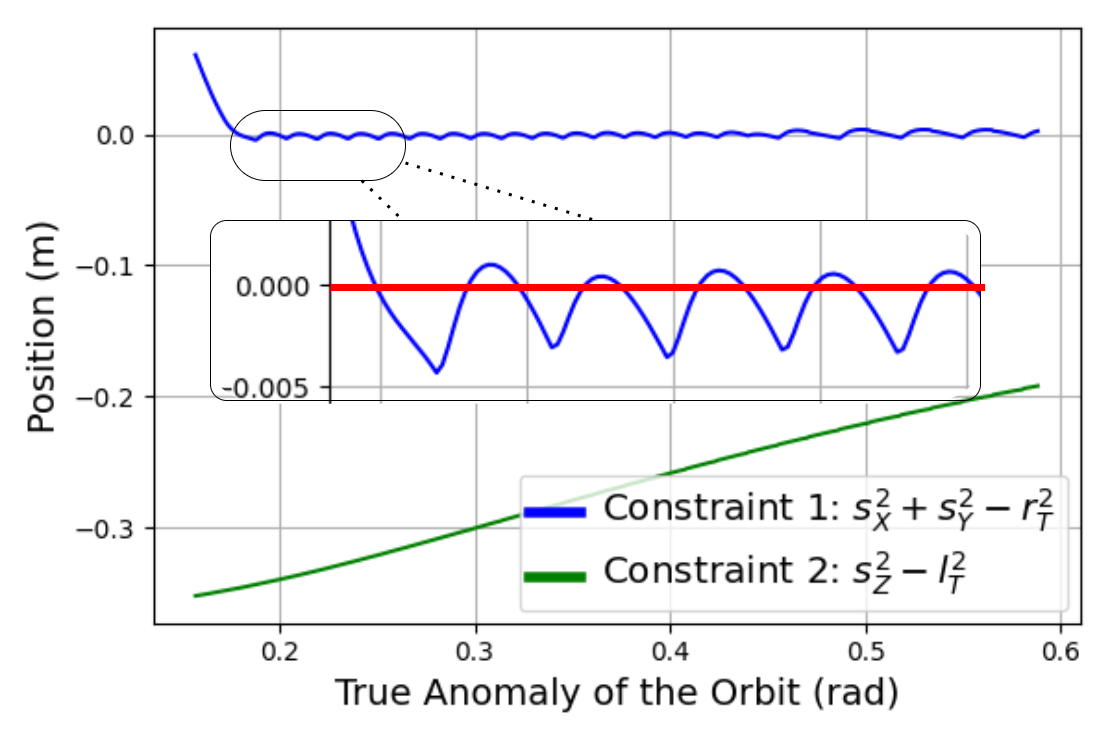
\includegraphics[width=\linewidth]{assets/results_no_tube_mpc.png}
    \caption{MPC (no robust tubes)}
    \label{fig:results_no_tube_mpc}
  \end{subfigure}
  \caption{Violation of Collision Constraints without Robust Tubes. With no robust tubes, there are several time periods when the collision constraint defined as $\boldsymbol{r}(\theta)\in{\mathcal{C}}_D$ is violated; i.e. when both Constraint 1 and Constraint 2 are less than zero.}
  \label{fig:results_tube}
\end{figure}
\subsection{Convergence to the desired docking position}
Although using dynamic tubes without adaptation proves to be effective in preventing collisions, the chaser is unable to converge to the desired docking position on the target due to inaccurate estimates of the unknown parameters and, hence, large robust tubes.
On the other hand, adaptive dynamic tube MPC shrinks the tube over time, hence allowing the chaser to converge to the final docking position.
Figure \ref{fig:results_adapt} demonstrates how, in very close proximity of the chaser to the target, the previous adaptation of unknown parameters and, hence, a smaller robust tube permits the chaser to move closer to the docking position.
\begin{figure}[H]
  \begin{subfigure}[b]{0.50\textwidth}
    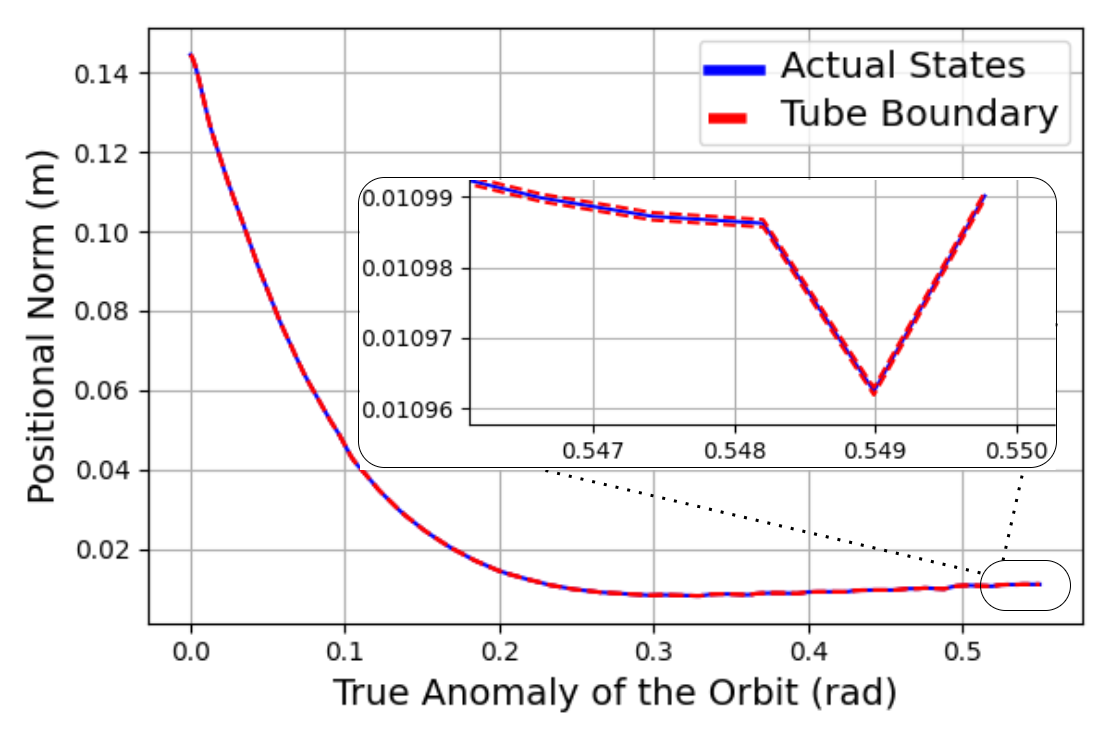
\includegraphics[width=\linewidth]{assets/results_adapt_adtmpc.png}
    \caption{Adaptive Dynamic Tube MPC}
    \label{fig:results_adapt_adtmpc}
  \end{subfigure}
  \hfill
  \begin{subfigure}[b]{0.50\textwidth}
    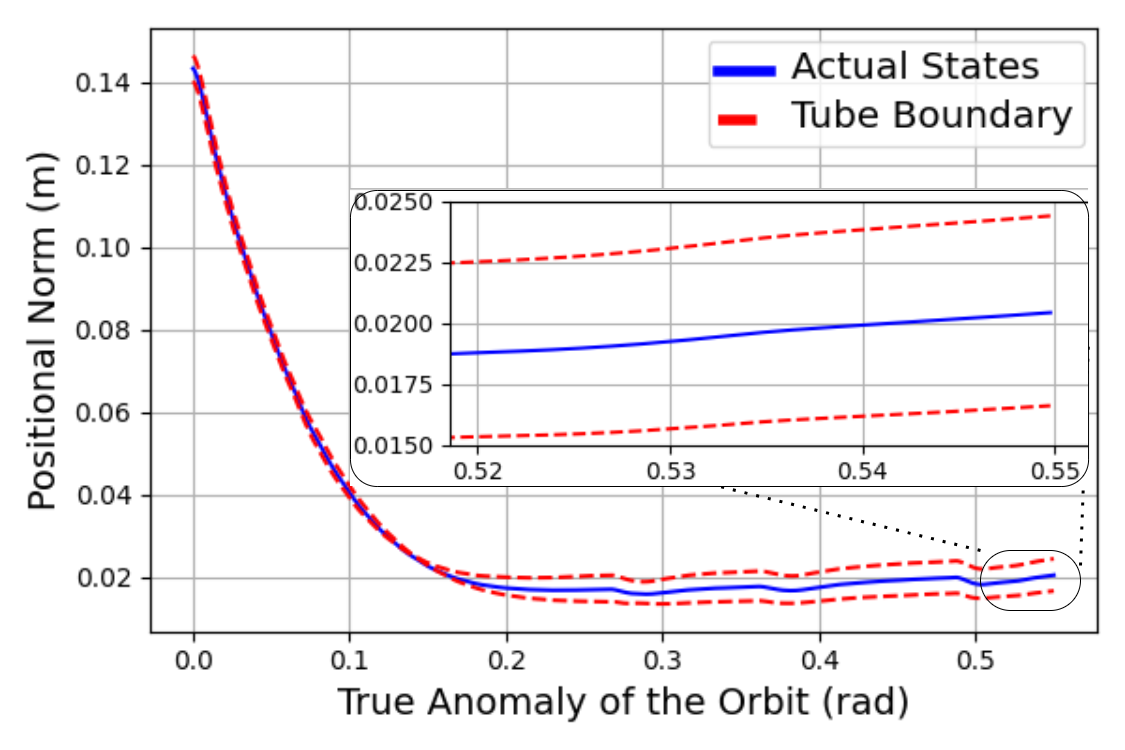
\includegraphics[width=\linewidth]{assets/results_adapt_dtmpc.png}
    \caption{Dynamic Tube MPC (no adaptation)}
    \label{fig:results_adapt_dtmpc}
  \end{subfigure}
  \caption{The Effect of Adaptation. These plots demonstrate the effect of SMID-based parameter estimation on the size of tubes and, hence, the convergence of the chaser to the final docking point.}
  \label{fig:results_adapt}
\end{figure}

\section{Target Deflection}
\label{sec:results_target_deflect}
Next, we run the optimization problem proposed in Section \ref{sec:target-deflection} such that the chaser attaches to a point within a set of known docking positions and applies a net optimal force to detumble the target.
We consider the target to be cylindrical in shape with a non-zero starting angular velocity.
The blue dot in figures \ref{fig:results_docking_point_unrestricted} (for the case with unrestricted docking points) and \ref{fig:results_docking_point_discretized} (for the case with discretized docking points) represents the optimal position of docking of the chaser on the target.
This point has been optimally calculated from a set of 24 points, 8 uniformly distributed on each circular boundary and 8 on the circle halfway between the boundary circles.
Figures \ref{fig:results_deflection_unrestricted} and \ref{fig:results_deflection_discretized} further demonstrate the trajectories of the angular position and the angular velocity of the target, and the forces applied by the chaser to stop its tumble.
\begin{table}[H]
    \centering
    \resizebox{\textwidth}{!}{\begin{tabular}{|c|c|c|c|}
        \hline
        & $\boldsymbol{\omega}_i$ (rad/s) & $\boldsymbol{\omega}_f$ (rad/s) & $||\boldsymbol{\omega}_f||$ (rad/s) \\
        \hline
        Unrestricted & $[-0.04, 0.10, -0.02]$ & $[\num{-9.614e-6}, \num{6.835e-6}, \num{-1.293e-7}]$ & $\num{1.180e-5}$ \\
        Discretized  & $[-0.04, 0.10, -0.02]$ & $[\num{-2.844e-3}, \num{7.571e-2}, \num{-2.402e-2}]$ & $\num{7.947e-2}$ \\
        \hline         
    \end{tabular}}
    \caption{Target Detumbling using Unrestricted and Discretized Docking Points}
    \label{tab:target_detumbling}
\end{table}
\begin{figure}[H]
  \centering
  \begin{subfigure}[b]{0.4\textwidth}
    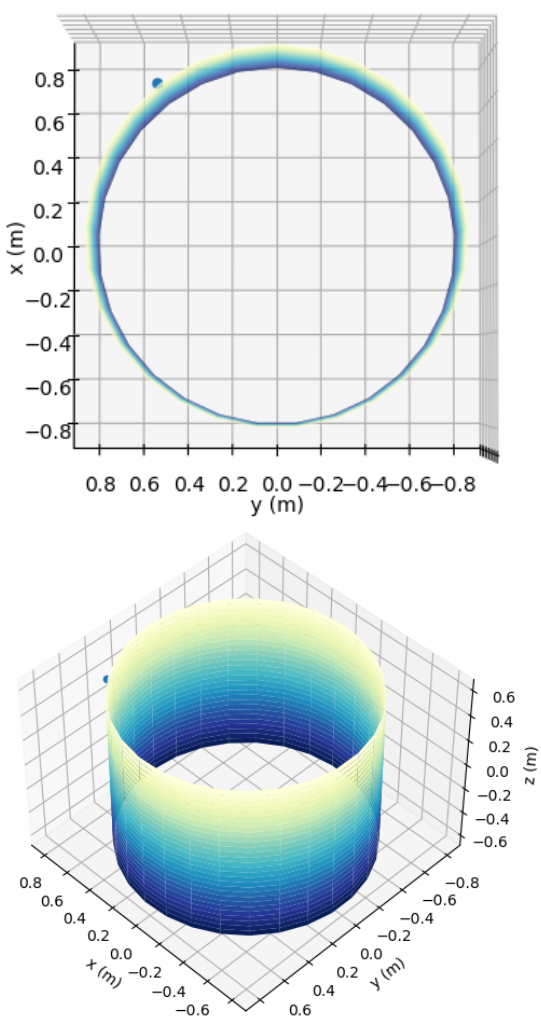
\includegraphics[width=\linewidth]{assets/results_docking_point_unrestricted_vert.png}
    \caption{Unrestricted Docking Points}
    \label{fig:results_docking_point_unrestricted}
  \end{subfigure}
  \begin{subfigure}[b]{0.4\textwidth}
    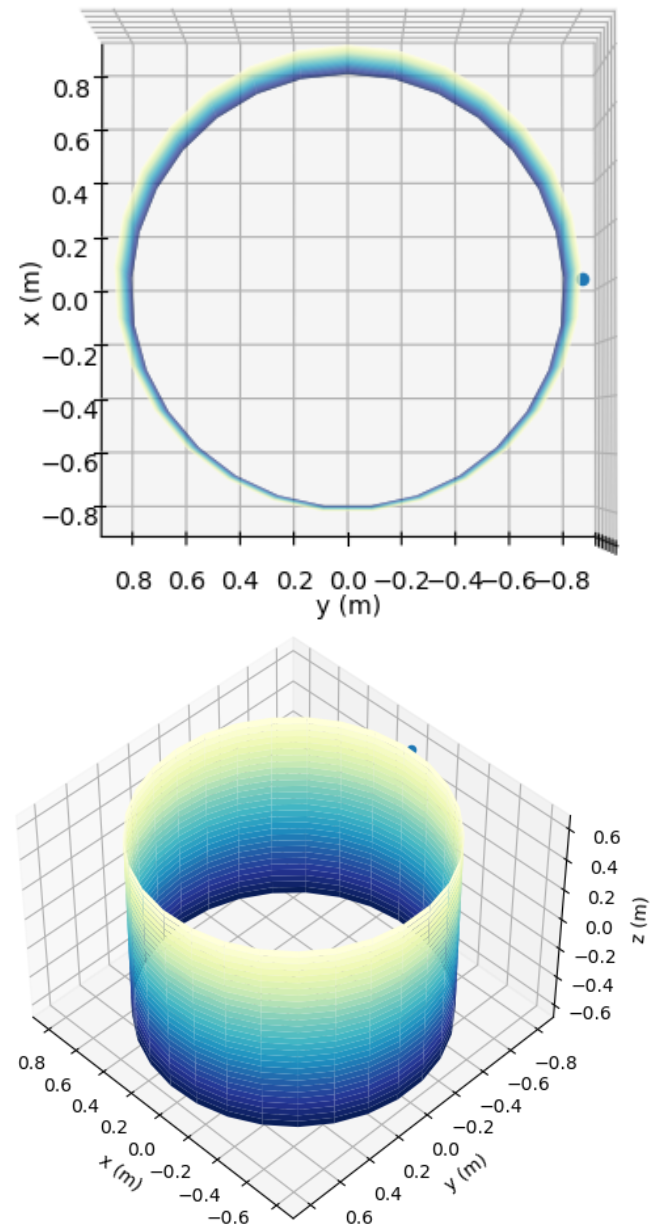
\includegraphics[width=\linewidth]{assets/results_docking_point_discretized_vert.png}
    \caption{Discretized Docking Points}
    \label{fig:results_docking_point_discretized}
  \end{subfigure}
  \caption{Optimal Chaser Docking Position}
  \label{fig:results_docking_point}
\end{figure}
It can be observed from Table \ref{tab:target_detumbling} that, with no restriction on the docking position of the chaser, the angular velocity of the target is brought to zero, hence stopping the tumble of the target.
The angular velocity of the target is significantly decreased even with discretized docking points.
This is also reflected in the convergence of the target angular position.
The unrestricted case provides a globally optimal position for docking whereas the discretized case picks the most optimal position from a finite set (in this case, a set of 48 points) which need not be the globally optimal position.
As a result, the force required to detumble the target is significantly larger for the latter case.
The docking positions are also different due to the discretization process and the subsequent difference in the initialization of the nonlinear dynamic optimization problem.
\section{Summary}
This chapter presents results on the simulation of rendezvous and docking of a single chaser with a cylindrical target in an elliptical orbit with drag.
It is shown that the implementation of dynamic tubes for robustness prevents inevitable collision with the target. 
Furthermore, the chapter demonstrates the accuracy of estimating the eccentricity of the orbit and the drag constant of the target.
This subsequently shrinks the robust tube around the trajectory of the chaser, hence making the trajectory less conservative.
Finally, the chapter presents results on the deflection of the target using chaser propulsion, comparing results for when any point on the target can be chosen for docking against the case with a discrete set of docking positions.
While the former case provides a globally optimal solution bringing the target to a standstill, the latter also significantly decreases the tumble of the target.
% \begin{figure}[H]
%     \centering
%     \includegraphics[width=0.95\linewidth]{assets/results_docking_point_unrestricted.png}
%     \caption{Optimal Chaser Docking Position with Unrestricted Docking Points}
%     \label{fig:results_docking_point_unrestricted}
% \end{figure}
% \begin{figure}[H]
%     \centering
%     \includegraphics[width=0.95\linewidth]{assets/results_docking_point_discretized.png}
%     \caption{Optimal Chaser Docking Position with Discretized Docking Points}
%     \label{fig:results_docking_point_discretized}
% \end{figure}


% UNRESTRICTED
% Position of the Chaser:  [0.63453837 0.49735406 0.6       ]
% Initial Angular Position: [ 0.0 0.2 -0.1 ]
% Initial Angular Velocity: [ -0.04 0.1 -0.02 ]
% Final   Angular Position: [ -0.0015024259646 0.20362891089 -0.10051285282 ]
% Final   Angular Velocity: [ -9.6140430806e-06 6.8354931586e-06 -1.2926002949e-07 ]
% Norm of Initial Angular Velocity:  0.10954451150103323
% Norm of Final   Angular Velocity:  1.1797054684628867e-05

% DISCRETIZED
% Position of the Chaser:  [-1.48628994e-06 -8.00000616e-01  6.00000240e-01]
% Initial Angular Position: [ 0.0 0.2 -0.1 ]
% Initial Angular Velocity: [ -0.04 0.1 -0.02 ]
% Final   Angular Position: [ -0.020816099278 0.22113934686 -0.058538949531 ]
% Final   Angular Velocity: [ -0.002844002 0.075705397522 -0.024016434397 ]
% Norm of Initial Angular Velocity:  0.10954451150103323
% Norm of Final   Angular Velocity:  0.07947442785252029
\begin{figure}[H]
  \centering
    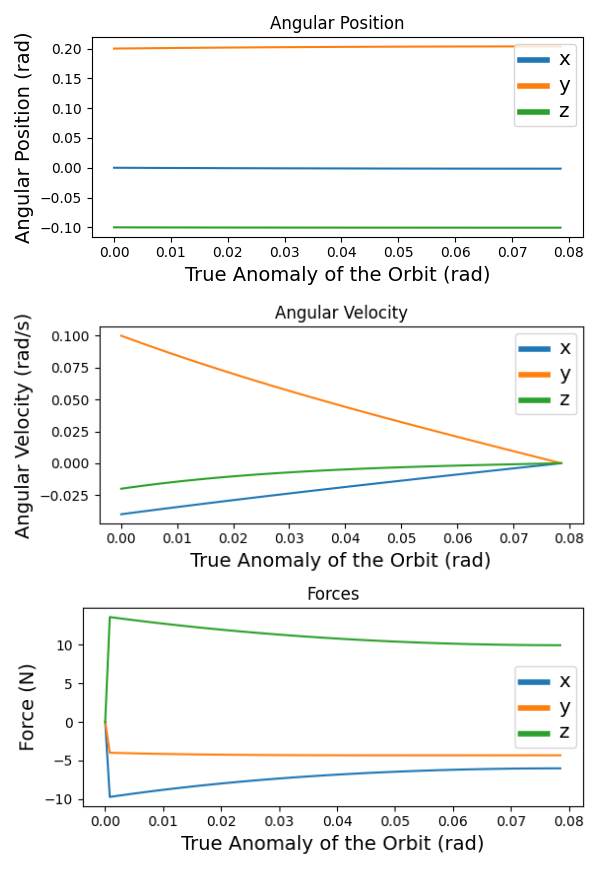
\includegraphics[width=0.8\linewidth]{assets/target_output_unrestricted.png}
  \caption{Detumbling of the Target and the Corresponding Chaser Control Effort with Unrestricted Docking Points.}
  \label{fig:results_deflection_unrestricted}
\end{figure}
\begin{figure}[H]
  \centering
    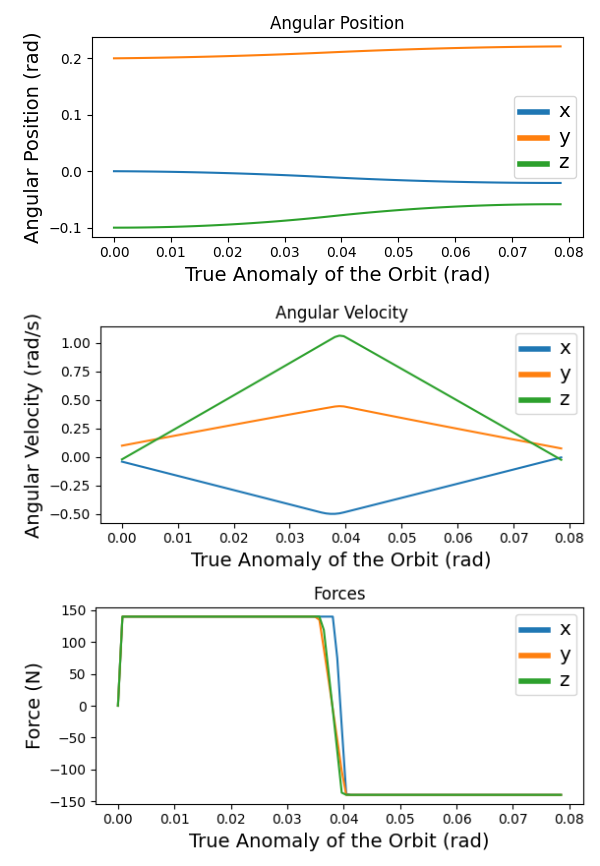
\includegraphics[width=0.8\linewidth]{assets/target_output_discretized.png}
  \caption{Detumbling of the Target and the Corresponding Chaser Control Effort with Discretized Docking Points.}
  \label{fig:results_deflection_discretized}
\end{figure}